\section{Einleitung}
%\lbrack Zitat (optional)\rbrack :
%\begin{quote}
%\glqq Was ist die Absicht eines wissenschaftlichen Buches? Es stellt Gedanken 
%dar und will den Leser von ihrer Gültigkeit überzeugen. Darüber hinaus will 
%der Leser auch wissen: woher kommen diese Gedanken und wohin führen sie? Mit 
%welchen Richtungen auf anderen Gebieten hängen sie zusammen?\grqq
%\pcite{}{XVII}{carnap1974}
%\end{quote}


Salesforce gehört laut \pcite{}{247}{softwareindustrie2015} zu den größten 
Software-as-a-Service-Anbietern und es wächst stetig weiter. 
Mit einem durchschnittlichen jährlichen Wachstum von 31\% konnte Salesforce 
seinen Umsatz von 2,267 Milliarden US-Dollar im Jahr 2012 auf 6,667 Milliarden 
US-Dollar im Jahr 2016 steigern. \ref{UmsatzzahlenSalesforce}


\begin{figure}[bh]
\begin{center}
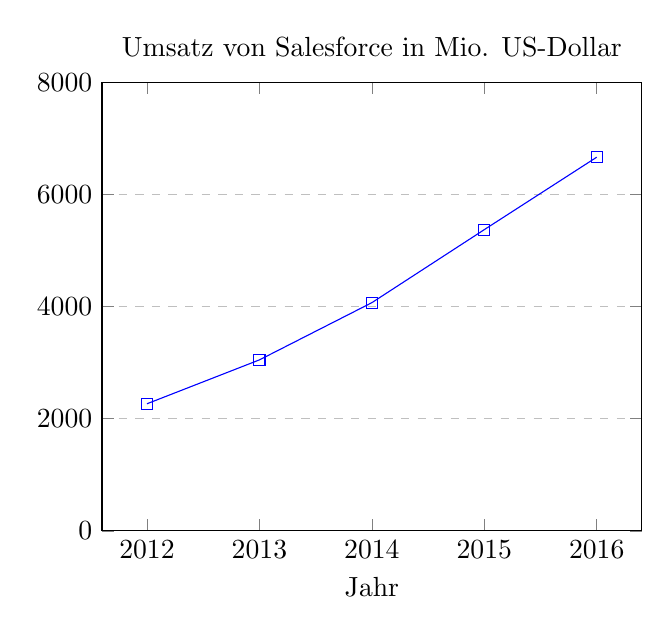
\begin{tikzpicture}
\begin{axis}[
/pgf/number format/.cd,
        use comma,
        1000 sep={},
    title={Umsatz von Salesforce in Mio. US-Dollar},
    xlabel={Jahr},
    %ylabel={Umsatz [Mio. US-Dollar]},
    %xmin=0, xmax=100,
    ymin=0, ymax=8000,
    %xtick={0,20,40,60,80,100},
    %ytick={0,20,40,60,80,100,120},
    legend pos=north west,
    ymajorgrids=true,
    grid style=dashed
]

\addplot[color=blue,mark=square,]
    coordinates {
    (2012,2267)(2013,3050)(2014,4071)(2015,5374)(2016,6667)
    };
    %\legend{Salesforce}
 
\end{axis}
\end{tikzpicture}
\caption{Umsatzzahlen entnommen aus \cite[43]{salesforceannualreport} }
\label{UmsatzzahlenSalesforce}

\end{center}
\end{figure}



Reply, das Unternehmen mit dem in Kooperation diese Bachelor-Thesis 
entstanden ist, ist ein an der italienischen Börse gehandeltes 
IT-Beratungsunternehmen und betrachtet sich 
als "`Living network"'\ aus hochspezialisierten Tochterunternehmen. Seit der 
Gründung 1996 konnte Reply seinen Umsatz auf über 705 Millionen Euro bei 5.245 
Angestellten im Jahr 2015 steigern. Das Netzwerk wuchs und wächst rasch: 
2016 wurden bis November drei neue Firmen aquiriert. Zwei 
Tochtergesellschaften, die schon seit mehreren Jahren Teil von Reply sind, 
möchte ich genauer vorstellen, da ihre Unternehmensprofile das 
Migrationsprojekt in dessen Rahmen diese Thesis entstanden ist, in besonderem 
Maße beeinflussen. \\
Die vormalige syskoplan AG, seit dem Erwerb 2010 \pcite{}{12}{replycompprofile} 
Syskoplan Reply, ist ein Spezialist für SAP-Applikationen und 
-Plattformen \pcite{}{10}{replycompprofile} und entwickelt seit 1999 das 
integrierte Facility Management System (iFMS). iFMS verbindet die in SAP 
hinterlegten Daten mit Gebäudeplänen und versucht Prozesse rund um die 
Verwaltung von Immobilien zu unterstützen. Die gewachsene 
Java-Anwendung mit einer Client-Server-Architektur lässt sich inzwischen nur 
noch schwer um von Kunden gewünschte Funktionen erweitern. Auch die Bedienung 
über 
eine zusätzlich zu installierenden Anwendung wirkt in Zeiten, in denen Nutzer 
es gewohnt sind, auch umfangreiche Software über den Webbrowser zu bedienen, 
anachronstisch. Beide Aspekte schränken die zukünftige
Wettbewerbsfähigkeit der Software ein. \\
Die ehemalige Arlanis Software AG wurde 2012 von Reply übernommen und ist 
Spezialist für Lösungen auf Basis des Cloud Anbieters Salesforce. 

Lösungen 
haben ganz allgemein zwei Vorteile für Unternehmen, die am für Salesforce 
typischen Beispiel einer Kundenverwaltung schildern möchte. Möchte ein 
Unternehmen Informationen zu seinen Kunden zentral speichern, muss es bei einer 
Cloudlösung keinen Server installieren und warten. Es kann also Kosten für 
Hardware sowie mindestens noch Personalkosten bei der Administration einsparen. 
Der erste Vorteil entsteht also durch Kosteneinsparungen auf Serverseite des 
Unternehmens. Cloudbasierte Software lässt sich regelmäßig mit einem Browser 
bedienen, der auf allen mobilen und internetfähigen Geräten wie auf 
herkömmlichen Computern verfügbar sein dürfte. Im Beispiel muss der Anwender, 
der Zugriff auf die Kundendaten nehmen will, keine Software installieren und 
ist an kein Gerät gebunden.\\
Die Idee hinter dem Migrationsprojekt ist die Verbindung der Expertise beider 
Unternehmen: Die Nutzung des aufgebauten Know-Hows auf einer neuen, 
zukunftsfähigen Plattform. \\
Dabei stellen sich die folgenden Fragen:
\begin{itemize}
	\item Welche Strategie sollte künftig mit dem bestehenden Produkt 
verfolgt werden?
	\item In welchem Umfang soll die Cloud Software durch 
	\begin{itemize}
		\item den Anbieter
		\item den Kunden
	\end{itemize}
	anpassbar sein?
	\item Wie lassen sich idealerweise die Anforderungen ermitteln?
	\item Welche Funktionen sollen übernommen werden?
	\item Wie lässt sich ein bestehendes Produkt an die neuen Möglichkeiten 
der Cloud anpassen?
\end{itemize}

Im folgenden gebe ich einen Überblick über Methoden des 
Requirements-Engineering.

